\chapter{Entorno de desarrollo}
\chaptermark{Entorno de desarrollo}

A la hora de seleccionar la plataforma para desarrollar las pruebas sobre los hipervisores Xen y Jailhouse se han barajado diferentes alternativas. Los criterios que se han tenido en cuenta para la selección han sido principalmente dos:
\begin{itemize}
  \item Plataformas soportadas: cada uno de los dos hipervisores mantiene una lista de plataformas en las que se ha probado alguna vez. Xen tiene un amplio recorrido en el mundo de los hipervisores y la lista de tarjetas electrónicas en las que se ha probado es muy grande. En el caso de Jailhouse, debido a que su trayectoria es más corta, esa lista de tarjetas soportadas se reduce enórmemente \cite{jailhouse_github}. La tarjeta seleccionada debía estar en las dos listas.
  \item Herramientas para generar máquinas virtuales: con el objeto de evaluar un sistema virtualizado con ambos hipervisores, se va a necesitar generar tanto un dominio o celda Linux con su kernel, device-tree y sistema de ficheros y un sistema baremetal. La selección de la tarjeta electrónica, o más bien la arquitectura del microprocesaro que incluya, marca también en gran medida las herramientas (compilador, BSP, etc.) para generar el software necesario. Cabe destacar que se le ha dado importancia al hecho de poder disponer de todo el código fuente que se vaya a utilizar para poder controlarlo, entenderlo y adaptarlo si fuera necesario.
\end{itemize}

Una de las arquitecturas más populares en los últimos tiempos en los sitemas embebidos es la arquitectura ARM. Es ubicua y en los ultimos años ha irrumpido con mucha fuerza. La famosa tarjeta de la frambuesa desde su inicio ha incluído un procesador ARM, lo que le ha dado más popularidad si cabe, y también Xilinx desde la familia Zynq\textregistered-7000 en su PS.\\
Debido a la familiaridad con las plataformas de Xilinx y sus herramientas y al creciente interés en la virtualización sobre la arquitectura ARMv8, se decidió optar por una tarjeta que incluyera un chip de la familia Zynq\textregistered UltraScale+\texttrademark. Además de esto, resulta de especial interés que además de incluir un procesador ARMv8 en la zona de PS, incluye una parte de PL o FPGA en la que se pueden desplegar diferentes periféricos con el objetivo de establecer un entono de pruebas y medidas flexible.

En el momento de iniciar el trabajo fin de máster no se disponía de la tarjeta Xilinx ZCU102, que aparece en la lista de plataformas soportadas en Xen y Jailhouse. En cambio, la platarforma que se podía utilizar era la UltraZed\texttrademark y debido a que incluye un chip de la familia Zynq\textregistered UltraScale+\texttrademark MPSoC al igual que la ZCU102, se estimó que las modificaciones necesarias para poder ejecutar ambos hipervisores no serían demasiado costosas, por lo que el desarrollo se ha efectuado sobre esa plataforma.

\section{Plataforma electrónica}
\subsection{Ultrazed}
La tarjeta electrónica que se ha utilizado se compone de dos partes: UltraZed-EG\texttrademark SOM y UltraZed\texttrademark IO Carrier Card con las siguientes características técnicas:
\begin{itemize}
  \item Procesador zu3egblablabal que inluye entre otras cosas:
  \begin{itemize}
    \item 4 núcleos ARM Cortex A53 (ARMv8)
  \end{itemize}
  \item 12 conectore PMOD conectados a la parte de PL
  \item 2 USB-UART
\end{itemize}

\begin{figure*}[h]
	\centering
	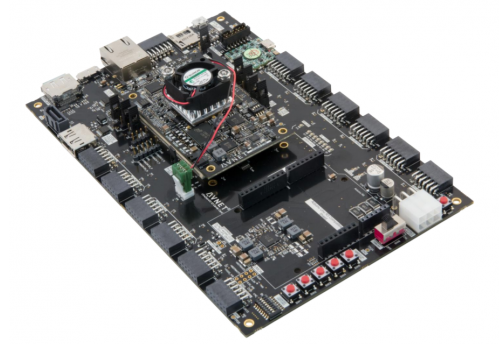
\includegraphics[width=0.65\textwidth]{recursos/ultrazed-eg-carrier.png}
	\caption{Hipervisor de tipo 1}
	\label{fig:ultrazed-eg-carrier}
\end{figure*}

UltraZed\texttrademark IO Carrier Card

\subsection{Otros}

\begin{itemize}
  \item Analizador lógico
  \item JTAG HS2
\end{itemize}

\section{Herramientas Software}
